\hypertarget{IU03}{\subsection{IU03 Página de empresa}}


    \subsubsection{Pantalla de datos}

    Después de presionar el botón para ver más información sobre una empresa,
    se abrirá una nueva pestaña en el navegador con sus datos.
    Primero se muestran los datos financieros (activos, pasivos y capital contable)
    con los que se han calculado las razones. Presione ``Editar registro''
    para modificar la información de la empresa.

    \begin{figure}[H]
        \begin{center}
            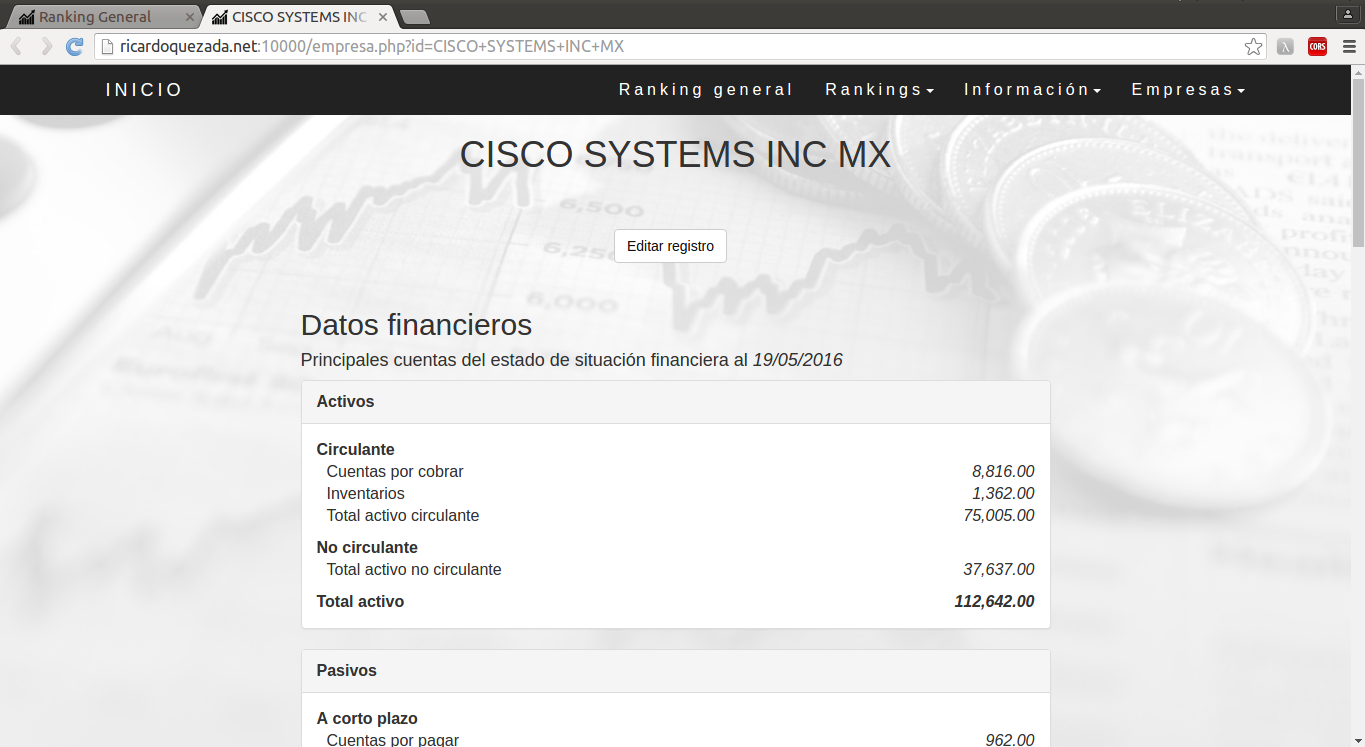
\includegraphics[scale=0.3]{pantallas/Empresa1}
            \caption{IU03/01 - Pantalla de datos}
        \end{center}
    \end{figure}


    \subsubsection{Pantalla de índices}

    Más abajo se encuentran las razones simples para dicha empresa,
    separados por índices. Cada índice tiene dos enlaces,
    uno para obtener información sobre ese índice y las razones que lo componen 
    y otro para ir al ranking de ese índice.

    \begin{figure}[H]
        \begin{center}
            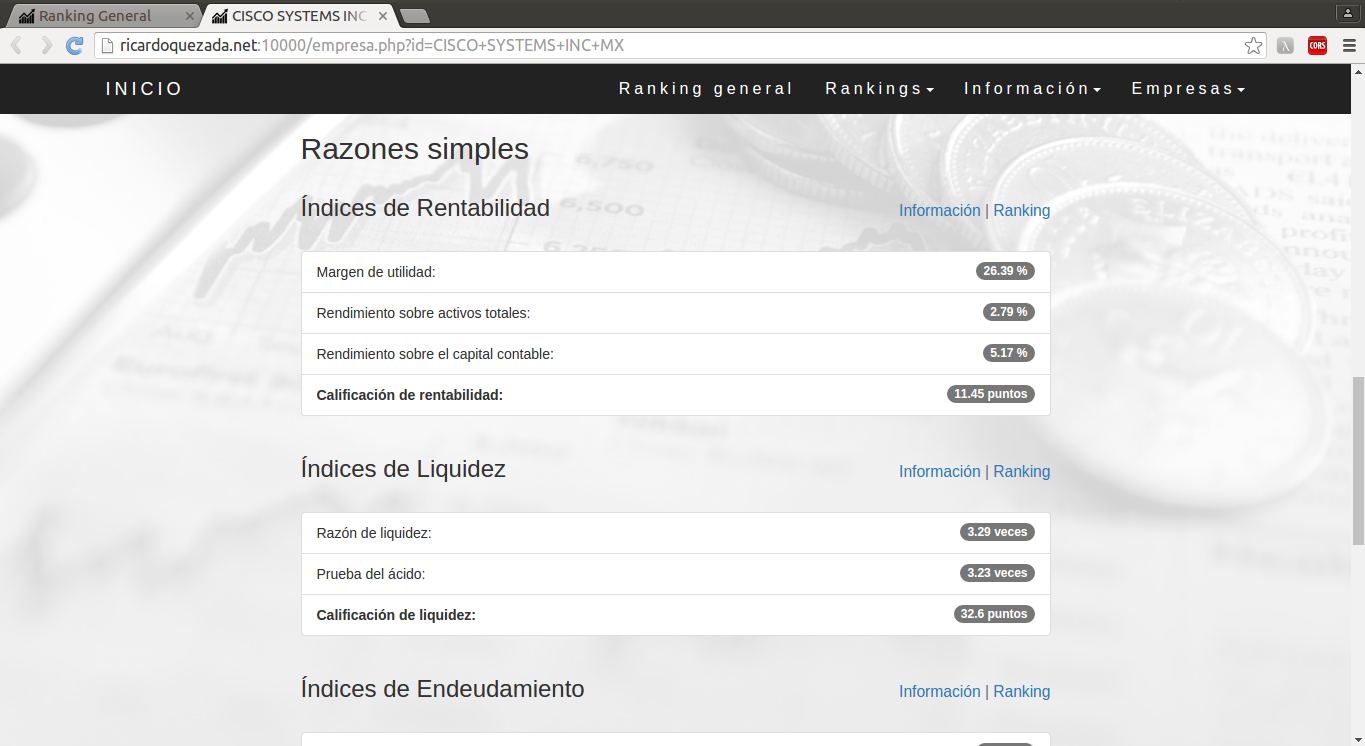
\includegraphics[scale=0.3]{pantallas/Empresa2}
            \caption{IU03/01 - Pantalla de índices}
        \end{center}
    \end{figure}
